\documentclass[
	% -- opções da classe memoir --
	12pt,				% tamanho da fonte
	openright,			% capítulos começam em pág ímpar (insere página vazia caso preciso)
	twoside,			% para impressão em verso e anverso. Oposto a oneside
	a4paper,			% tamanho do papel. 
	% -- opções da classe abntex2 --
	%chapter=TITLE,		% títulos de capítulos convertidos em letras maiúsculas
	%section=TITLE,		% títulos de seções convertidos em letras maiúsculas
	%subsection=TITLE,	% títulos de subseções convertidos em letras maiúsculas
	%subsubsection=TITLE,% títulos de subsubseções convertidos em letras maiúsculas
	% -- opções do pacote babel --
	english,			% idioma adicional para hifenização
	brazil				% o último idioma é o principal do documento
	]{abntex2}

    % ---
% Pacotes básicos 
% ---
\usepackage{lastpage}			% Usado pela Ficha catalográfica
\usepackage{indentfirst}		% Indenta o primeiro parágrafo de cada seção.
\usepackage{color}				% Controle das cores
\usepackage{graphicx}			% Inclusão de gráficos
\usepackage{microtype} 			% para melhorias de justificação

% pacotes adicionados
\usepackage{amsmath}
\usepackage{amssymb,amsfonts,amsthm}
\usepackage{setspace}
% ---
		
% ---
% Pacotes adicionais, usados apenas no âmbito do Modelo Canônico do abnteX2
% ---
\usepackage{lipsum}				% para geração de dummy text
% ---
\usepackage{todonotes}
% ---
% Pacotes de citações
% ---
\usepackage[brazilian,hyperpageref]{backref}	 % Paginas com as citações na bibl
\usepackage[alf]{abntex2cite}	% Citações padrão ABNT


\renewcommand{\bf}[1]{\mathbf{#1}}
\renewcommand{\rm}[1]{\mathrm{#1}}


\usepackage{cite}
\renewcommand\citeleft{[}
\renewcommand\citeright{]}


% ---
% Configurações de aparência do PDF final

% alterando o aspecto da cor azul
\definecolor{blue}{RGB}{41,5,195}

% informações do PDF
\makeatletter
\hypersetup{
     	%pagebackref=true,
		colorlinks=true,       		% false: boxed links; true: colored links
    	linkcolor=blue,          	% color of internal links
    	citecolor=black,        		% color of links to bibliography
    	filecolor=magenta,      		% color of file links
		urlcolor=blue,
		bookmarksdepth=4
}



\makeatother
% --- 

% --- 
% Espaçamentos entre linhas e parágrafos 
% --- 

% O tamanho do parágrafo é dado por:
\setlength{\parindent}{1.3cm}

% Controle do espaçamento entre um parágrafo e outro:
\setlength{\parskip}{0.2cm}  % tente também \onelineskip

% ---
% compila o indice
% ---
\makeindex
% ---

% ----
% Início do documento
% ----
\begin{document}

% Seleciona o idioma do documento (conforme pacotes do babel)
%\selectlanguage{english}
\selectlanguage{brazil}
\graphicspath{ {./images/} }



\chapter{\textit{Modelagem dinâmica}}


\section{Modelagem do quadrirrotor}

Para se estudar as características de movimento e o sistema de controle do quadrirrotor deste trabalho é necessário entender como as forças que interagem com o corpo se relacionam. Assim, neste capítulo será apresentado essa análise.

\subsection{Sistemas de coordenadas}

Podemos modelar um quadrirrotor considerando-o como um corpo rígido usando as leis de newton, que necessitam de um referencial inercial(que não está acelerando nem rotacionando) para serem válidas, bem como definir um sistema de coordenadas local que se move com o quadrirrotor.
Nesse estudo, por conveniência escolhemos como sistema de coordenadas inercial o sistema North, East, Down(NED), que é tangencial a superfície da Terra e têm o eixo x apontando para o norte, o eixo y apontando para o leste e o eixo z apontando para baixo. E como sistema de coordenadas local um sistema ABC(Aircraft body centered) com origem no centro de gravidade do quadrirrotor e paralelo ao sistema NED.

\begin{figure}[h]
	\centering
	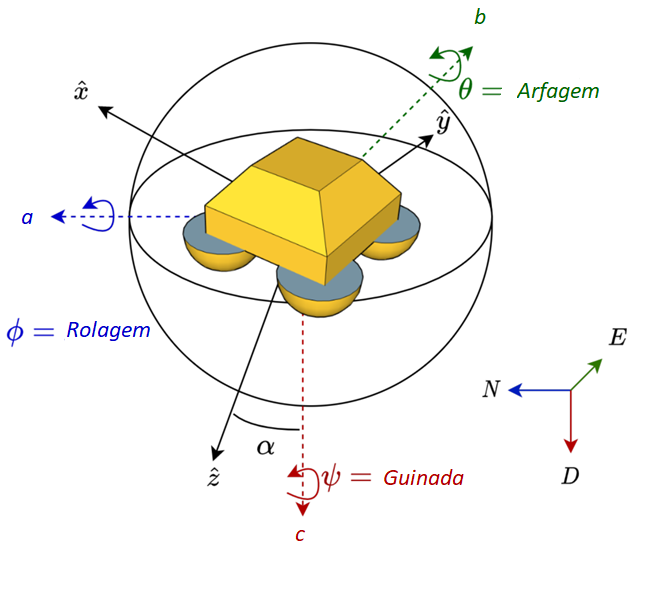
\includegraphics[width=0.6\textwidth]{nedxabc-reference}
	\caption{Representação do sistema de referência inercial(NED) e do sistema local ABC. Imagem retirada de https://www.mdpi.com/1424-8220/21/4/1310/html e modificada pelo autor.}
	\centering
	\label{figure-quadricopter}
\end{figure}


\subsection{Matrizes de rotação}
A fim de realizar a modelagem dinâmica do quadrirrotor se faz necessário relacionar o sistema de referência inercial(NED), que será nosso sistema de trabalho, com o sistema de referência do corpo(XYZ) obtendo assim a matriz de rotação entre os sistemas, que chamaremos de Rib.
A matriz de rotação Rib é obtida através de 3 rotações sucessivas ao longo dos eixos do sistema inercial, assim a sequência utilizada nesse trabalho será a x-y-z, ou seja, uma rotação de ($\phi$) ao longo do eixo x (rolagem), uma rotação ($\theta$) ao longo do eixo y (arfagem) e uma rotação ($\psi$) ao longo do eixo z (guinada).
Cada rotação pode ser representada a partir de uma matriz, sendo que, a  matriz de rotação ao longo de x é:




\begin{equation*}
	R_x = \begin{pmatrix}
		1 & 0         & 0        \\
		0 & \cos\phi  & \sin\phi \\
		0 & -\sin\phi & \cos\phi
	\end{pmatrix}
\end{equation*}

A  matriz de rotação ao longo de y é:

\begin{equation*}
	R_y = \begin{pmatrix}
		\cos\theta  & 0 & \sin\theta \\
		0           & 1 & 0          \\
		-\sin\theta & 0 & \cos\theta
	\end{pmatrix}
\end{equation*}

A  matriz de rotação ao longo de z é:

\begin{equation*}
	R_z = \begin{pmatrix}
		\cos\psi  & 0        & \sin\psi \\
		-\sin\psi & \cos\psi & 0        \\
		0         & 0        & 1
	\end{pmatrix}
\end{equation*}

	\includegraphics[width=1\textwidth]{matrix-rotation-explained}


Tais rotações podem ser melhor observadas na figura \ref{fig:matrix-rotation-explained}.

A matriz de transformação de referência  Rib que relaciona os dois sistemas de referencia, inercial e fixo ao corpo, é o produto das matrizes Rx, Ry, Rz. De forma que:


\[
  R_{t}(\phi,\theta,\psi) = R_z(\psi) R_y(\theta) R_x(\phi) = 
  \begin{bmatrix}
    c_\theta c_\psi & s_\phi s_\theta c_\psi - c_\phi s_\psi & c_\phi s_\theta c_\psi + s_\phi s_\psi \\
    c_\theta s_\psi & s_\phi s_\theta s_\psi + c_\phi c_\psi & c_\phi s_\theta s_\psi - s_\phi c_\psi \\
    -s_\theta & s_\phi c_\theta & c_\phi c_\theta
  \end{bmatrix}
\]


\subsection{Configuração do veículo}


Observando o diagrama de corpo livre do quadricóptero retratado pela figura \ref*{figure-quadricopter},
chega-se nos seis graus de liberdade necessários para a representação do sistema. Esses se
dividem em três para o movimento de translação nos eixos x’, y’ e z’ e outros três para
o movimento de rotação em cada um dos eixos. Para melhor estudo do problema, foram
estabelecidos um referencial inercial e um referencial solidário ao corpo relacionados da
seguinte forma:

\begin{align*}
	\begin{bmatrix}
		x \\
		y \\
		z \\
	  \end{bmatrix}
	&= R_t
		\begin{bmatrix}
			x’ \\
			y’ \\
			z’ \\
		  \end{bmatrix}
  \end{align*}



Na sequência,  usaremos a matriz de rotação previamente obtida, para descrever a rotação o movimento geral do corpo a partir de suas equações de movimento translacional e rotacional.

Pode-se utilizar da matriz de rotação RT para chegar na seguinte relação entre as
velocidades:


\begin{align*}
	\begin{bmatrix}
		$$ \dot{x} $$ \\
		$$ \dot{y} $$ \\
		$$ \dot{z} $$ \\
	  \end{bmatrix}
	&= R_t
		\begin{bmatrix}
			u \\
			v \\
			w \\
		  \end{bmatrix}
  \end{align*}

Para a análise da dinâmica rotacional do movimento, podemos utilizar as equações XX-XX, historicamente conhecidas como equações de Euler(HIBBLER), essas equações consideram que o sistema de referência solidário ao corpo é coincidente com o centro de massa e o corpo é rígido e simétrico, fazendo que os produtos de inércia sejam zero, Ixx = Ix, Iyy = Iy, Izz = Iz:

\begin{equation*}
	I = \begin{pmatrix}
		I_{xx}  & 0      & 0 \\
		0       & I_{yy} & 0   \\
		0       & 0      & I_{zz}
	\end{pmatrix}
\end{equation*}

Onde Ixx, Iyy e Izz são os momentos de inércia sobre os seus eixos principais.

Usando a Segunda Lei de Newton, podemos expressar a soma dos momentos atuantes em um corpo como:

\[ \vec{M} = \dot{\vec{H}} \ \ \ (2.9) \]

Nesta equação, \(\vec{H}\) denota o momento angular. O momento angular total de um quadrirotor compreende duas componentes distintas. A primeira delas diz respeito à rotação do próprio corpo, enquanto a segunda está relacionada à rotação dos motores. Portanto,

\[ \vec{H} = \vec{H}_{\text{corpo}} + \vec{H}_{\text{motores}} \ \ \ (2.10) \]

Onde \(\vec{H}_{\text{corpo}}\) representa o momento angular do corpo e \(\vec{H}_{\text{motores}}\) corresponde ao momento angular devido aos motores. Esses momentos angulares podem ser descritos da seguinte forma:

\[ \vec{H}_{\text{corpo}} = \vec{I}_{\text{corpo}} \cdot \vec{\omega}_{\text{corpo}} \ \ \ (2.11) \]

\[ \vec{H}_{\text{motores}} = \begin{bmatrix} 0 \\ 0 \\ J_r \Omega \end{bmatrix} \ \ \ (2.12) \]

Aqui, \(J_r\) representa o momento de inércia do conjunto composto pelo rotor, eixo e hélice, enquanto \(\Omega\) é a velocidade nominal de rotação do motor. Portanto, a equação de Euler que descreve a dinâmica de rotação é definida como:

\[ \dot{\vec{I}_{\text{corpo}} \cdot \vec{\omega}_{\text{corpo}}} = \vec{M} - \vec{\omega}_{\text{corpo}} \times (\vec{H}_{\text{corpo}} + \vec{H}_{\text{motores}}) \ \ \ (2.13) \]

Os termos \(\dot{\vec{I}_{\text{corpo}}  \vec{\omega}_{\text{corpo}}}\)    e    \(\vec{\omega}_{\text{corpo}} \times (\vec{H}_{\text{corpo}} + \vec{H}_{\text{motores}})\) representam a taxa de variação do momento angular no sistema do corpo. O operador de produto vetorial \(\times\) é aplicado na última parte da equação.


\subsection(Cinemática de Rotação)


%---------------------------------------------------------------------
% INDICE REMISSIVO
%---------------------------------------------------------------------
\phantompart
\printindex
%---------------------------------------------------------------------

\end{document}
